\section{Conclusion}

\subsection{Summary}
\begin{frame}{Summary}
	\begin{itemize}
		\item
		allocation:
		partition of items amongst agents

		\item
		bundles valued using submodular valuation functions
		\begin{itemize}
			\item
			diminishing returns
		\end{itemize}

		\item
		Nash social welfare:
		weighted geometric mean of valuations

		\item
		approximation factor independent from \(m\)?

		\item
		simple, repeated matching fails because of missing foresight

		\item
		\RepReMatch:
		\(2n (\log n + 3)\)-approximative
		\begin{description}
			\item[Phase \phasei]
			finding enough outstanding items

			\item[Phase \phaseii]
			assigning remaining item

			\item[Phase \phaseiii]
			assigning outstanding items
		\end{description}
	\end{itemize}
	\beamerimage at (13cm,  5.00cm) {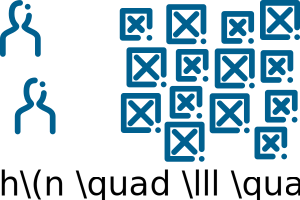
\includegraphics[height=1.45cm]{img/nvsm}};
	\beamerimage at (13cm,  3.25cm) {\includegraphics[height=1.45cm]{img/allocation}};
	\beamerimage at (13cm,  1.50cm) {\includegraphics[height=1.45cm]{img/outstanding_1}};
	\beamerimage at (13cm, -0.25cm) {\includegraphics[height=1.45cm]{img/anal2_1}};
%	\begin{center}
%		\includegraphics[height=2cm]{img/n_vs_m}
%		\hfil
%		\begin{tikzpicture}[scale=0.3, transform shape, every node/.style={minimum size=5mm}, node distance=10mm and 32mm]
%				% items
%				\node[draw, rectangle] (i1)                {};
%				\node[draw, rectangle] (i2)  [below=of i1] {};
%				\node[draw, rectangle] (i3)  [below=of i2] {};
%				\node[draw, rectangle] (im)  [below=of i3] {};
%				\node[draw, rectangle] (im1) [below=of im] {};
%				% agents
%				\node[draw, circle] (a1) [left=of i1]  {};
%				\node[draw, circle] (a2) [left=of im1] {};
%				% valuations
%				\draw (a1) to (i1);
%				\draw (a1) to (i2);
%				\draw (a1) to (i3);
%				\draw (a1) to (im);
%				\draw (a1) to (im1);
%
%				\draw (a2) to (i1);
%				\draw (a2) to (i2);
%				\draw (a2) to (i3);
%				\draw (a2) to (im);
%				\draw (a2) to (im1);
%		\end{tikzpicture}
%		\hfil
%		\includegraphics[height=2cm, page=19]{example-image-duck}
%		\hfil
%		\includegraphics[height=2cm]{img/anal2_1}
%	\end{center}
\end{frame}





\subsection{Outlook}
\begin{frame}{Outlook}
	An improvement over previous results?

	Yes!
	\((m-n+1)\) best known approximation factor before.

	\medskip

	Any room for improvement left?

	Possibly!
	Lower bound of \(1.72\).

	\bigskip

	Other approaches:
	\begin{itemize}
		\item
		less general valuation functions \(\leadsto\) better factors

		\item
		limits on agent weights \(\leadsto\) linear and even constant factors
	\end{itemize}
\end{frame}





\begin{frame}[c, plain, noframenumbering]
	\renewcommand{\insertsectionnumber}{!}
	\renewcommand{\insertsection}{End of Talk}
	\sectionpage
\end{frame}